\section{LES LIAISONS CINÉMATIQUES}\TLSectionLabel{3}

\subsection{Introduction}

Une liaison est un \textbf{modèle du comportement cinématique} d'un solide
par rapport à un autre. Elle définit les mouvements relatifs possibles,
indépendamment de la réalisation technologique : contact direct, coussinet,
roulement, etc.

\begin{center}
\begin{minipage}{.56\linewidth}
Différentes réalités technologiques peuvent donc conduire au même
comportement cinématique et à la même liaison.
\end{minipage}\hfill
\begin{minipage}{.40\linewidth}\centering
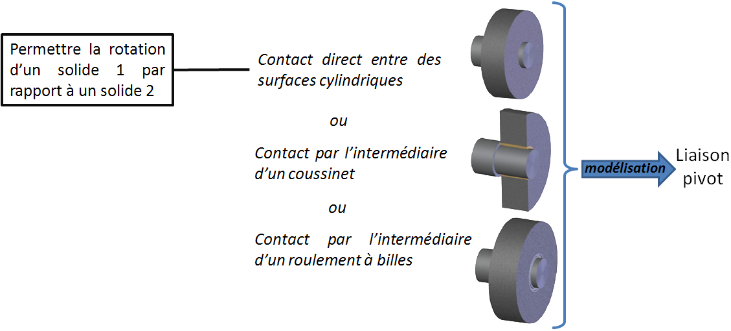
\includegraphics[width=\linewidth,height=.20\textheight,keepaspectratio]{images/image19.png}
\end{minipage}
\end{center}

\subsection{Degrés de liberté}

\begin{TLDefinition}
Un \textbf{degré de liberté} est un mouvement relatif élémentaire indépendant
autorisé par une liaison. Les six mouvements élémentaires sont les trois
translations \(T_x,T_y,T_z\) et les trois rotations \(R_x,R_y,R_z\).
\end{TLDefinition}

\begin{center}
\begin{tabular}{|c|p{.60\linewidth}|}
\hline
\rowcolor{TLTableHeader}\textbf{Mouvement} & \textbf{Signification}\\ \hline
\(T_x,T_y,T_z\) & translations rectilignes suivant \(\vec x,\vec y,\vec z\)\\ \hline
\(R_x,R_y,R_z\) & rotations autour des axes \((O,\vec x),(O,\vec y),(O,\vec z)\)\\ \hline
\end{tabular}\qquad

\includegraphics[width=.22\linewidth,height=.17\textheight,keepaspectratio]{images/image26.png}
\end{center}

Le nombre de degrés de liberté est le nombre de paramètres indépendants
nécessaires pour caractériser le mouvement relatif entre les deux solides.

\subsection{Description d'une liaison}

Pour chacune des liaisons, on associe les informations suivantes.

\begin{tabularx}{\linewidth}{|>{\bfseries}p{.28\linewidth}|X|}
\hline
\rowcolor{TLTableHeader}Élément & Remarques\\ \hline
Nom & Deux désignations peuvent parfois correspondre à une même liaison.\\ \hline
Description géométrique & Axe pour un cylindre, normale pour un plan, centre pour une sphère.\\ \hline
Symboles 2D et 3D & Ils expriment uniquement les mouvements possibles et non la réalisation matérielle.\\ \hline
Mobilités / degrés de liberté & Tableau des rotations et translations autorisées.\\ \hline
Paramétrage & Position linéaire ou angulaire relative ; les rotations sont représentées sur une figure de changement de base.\\ \hline
Torseur cinématique & Forme générale exprimée en un point caractéristique de la liaison.\\ \hline
\end{tabularx}

\subsection{Liaisons simples}

Les liaisons simples proviennent de l'association de surfaces élémentaires :
plan, cylindre et sphère.

\begin{center}
\begin{tabularx}{.96\linewidth}{|c|>{\centering\arraybackslash}X|>{\centering\arraybackslash}X|>{\centering\arraybackslash}X|}
\hline
 & \textbf{Plan} & \textbf{Sphère} & \textbf{Cylindre}\\ \hline
\textbf{Plan}
& 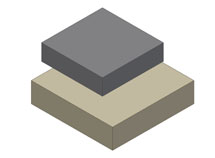
\includegraphics[width=.55\linewidth]{images/image37.jpeg}\\Appui-plan\\contact surfacique
& 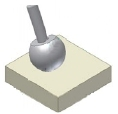
\includegraphics[width=.55\linewidth]{images/image38.jpeg}\\Sphère-plan\\contact ponctuel
& 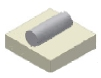
\includegraphics[width=.55\linewidth]{images/image39.jpeg}\\Cylindre-plan\\contact linéique\\ \hline
\textbf{Sphère}
& 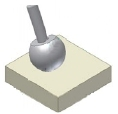
\includegraphics[width=.55\linewidth]{images/image38.jpeg}\\Sphère-plan
& 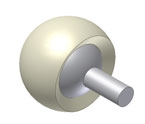
\includegraphics[width=.55\linewidth]{images/image40.jpeg}\\Sphérique
& 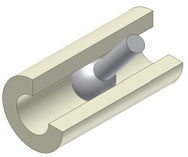
\includegraphics[width=.55\linewidth]{images/image41.jpeg}\\Sphère-cylindre\\ \hline
\textbf{Cylindre}
& 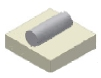
\includegraphics[width=.55\linewidth]{images/image39.jpeg}\\Cylindre-plan
& 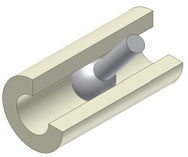
\includegraphics[width=.55\linewidth]{images/image41.jpeg}\\Sphère-cylindre
& 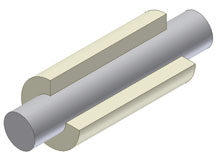
\includegraphics[width=.55\linewidth]{images/image42.jpeg}\\Pivot glissant\\ \hline
\end{tabularx}
\end{center}

\begin{longtable}{|p{.22\linewidth}|>{\centering\arraybackslash}p{.15\linewidth}|p{.15\linewidth}|p{.34\linewidth}|}
\hline
\rowcolor{TLTableHeader}
\textbf{Liaison} & \textbf{Symbole} & \textbf{Mobilité} & \textbf{Torseur cinématique}\\ \hline
\endfirsthead
\hline\rowcolor{TLTableHeader}
\textbf{Liaison} & \textbf{Symbole} & \textbf{Mobilité} & \textbf{Torseur cinématique}\\ \hline
\endhead
Appui-plan de normale \(\vec z\) &
\TLSymAppuiPlan &
\(R_z,T_x,T_y\) — 3 ddl &
\TLTorseur{\omega_x}{\omega_y}{\omega_z}{v_x}{v_y}{0}{P,\mathcal B}\\ \hline
Sphère-plan de normale \(\vec z\) &
\TLSymSpherePlan &
\(R_x,R_y,R_z,T_x,T_y\) — 5 ddl &
\TLTorseur{\omega_x}{\omega_y}{\omega_z}{v_x}{v_y}{0}{P,\mathcal B}\\ \hline
Sphère-cylindre d'axe \(\vec z\) &
\TLSymSphereCylindre &
4 ddl &
\TLTorseur{\omega_x}{\omega_y}{\omega_z}{0}{0}{v_z}{O,\mathcal B}\\ \hline
Cylindre-plan d'axe \(\vec x\), normale \(\vec z\) &
\TLSymCylindrePlan &
4 ddl &
\TLTorseur{\omega_x}{0}{\omega_z}{v_x}{v_y}{0}{P,\mathcal B}\\ \hline
Sphérique de centre \(O\) &
\TLSymSpherique &
\(R_x,R_y,R_z\) — 3 ddl &
\TLTorseur{\omega_x}{\omega_y}{\omega_z}{0}{0}{0}{O,\mathcal B}\\ \hline
Pivot glissant d'axe \(\vec z\) &
\TLSymPivotGlissant &
\(R_z,T_z\) — 2 ddl &
\TLTorseur{0}{0}{\omega_z}{0}{0}{v_z}{P,\mathcal B}\\ \hline
\end{longtable}

\TLReflectionBox{Compléter le tableau de mobilités et les symboles manquants, puis vérifier la cohérence avec les formes générales des torseurs cinématiques.}

\subsection{Liaisons composées}

Les liaisons composées résultent de plusieurs contacts élémentaires en série
ou en parallèle : glissière, pivot, hélicoïdale et sphérique à doigt.

\begin{center}
\begin{tabular}{cccc}
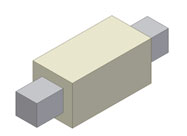
\includegraphics[width=.18\linewidth]{images/image61.jpeg} &

\includegraphics[width=.18\linewidth]{images/image62.jpeg} &
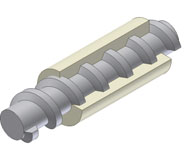
\includegraphics[width=.18\linewidth]{images/image63.jpeg} &
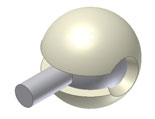
\includegraphics[width=.18\linewidth]{images/image64.jpeg}\\
\textbf{Glissière} & \textbf{Pivot} & \textbf{Hélicoïdale} & \textbf{Sphérique à doigt}
\end{tabular}
\end{center}

\begin{longtable}{|p{.22\linewidth}|>{\centering\arraybackslash}p{.15\linewidth}|p{.15\linewidth}|p{.34\linewidth}|}
\hline
\rowcolor{TLTableHeader}
\textbf{Liaison} & \textbf{Symbole} & \textbf{Mobilité} & \textbf{Torseur cinématique}\\ \hline
\endfirsthead
\hline\rowcolor{TLTableHeader}
\textbf{Liaison} & \textbf{Symbole} & \textbf{Mobilité} & \textbf{Torseur cinématique}\\ \hline
\endhead
Glissière de direction \(\vec z\) &
\TLSymGlissiere &
\(T_z\) — 1 ddl &
\TLTorseur{0}{0}{0}{0}{0}{v_z}{P,\mathcal B}\\ \hline
Pivot d'axe \((O,\vec z)\) &
\TLSymPivot &
\(R_z\) — 1 ddl &
\TLTorseur{0}{0}{\omega_z}{0}{0}{0}{P,\mathcal B}\\ \hline
Hélicoïdale d'axe \((O,\vec z)\) &
\TLSymHelicoidale &
\(R_z,T_z\) liés — 1 ddl &
\(v_z=p\,\omega_z\), avec \(p\) le pas réduit\\ \hline
Sphérique à doigt de centre \(O\), rotation \(\vec z\) interdite &
\TLSymSpheriqueDoigt &
2 ddl &
\TLTorseur{\omega_x}{\omega_y}{0}{0}{0}{0}{O,\mathcal B}\\ \hline
\end{longtable}

\begin{TLQuoteBox}
Pour un appui-plan, la seule rotation autorisée est celle autour de la
normale. Pour une liaison cylindre-plan, la seule translation impossible
est celle suivant la normale.
\end{TLQuoteBox}

% -----------------------------------------------------------------------------
